\documentclass{article}
\usepackage{array}
\usepackage[margin=1in]{geometry}
\usepackage{graphicx}
\graphicspath{ {./images/} }

\newcolumntype{C}[1]{>{\centering\let\newline\\\arraybackslash\hspace{0pt}}m{#1}}

\begin{document}
	
	\title{Permanent Magnet Alternating Current Motor Controller}
	\author{Alex Simon}
	
	\maketitle
	
	\begin{abstract}
		This document explores the design decisions for a Permanent Magnet Alternating Current (PMAC) motor controller.  Specifically, the hardware component design choices and the commutation techniques used within the project.
	\end{abstract}
	
	\section{Introduction}
	This paper will explore the process of designing a PMAC motor controller and the difficulties discovered along the way.  Beginning with the printed circuit board (PCB) design stage, each of the major components used in the PCB will be evaluated.  Once the PCB has been designed two different commutation techniques will be explored.  Trapezoidal commutation will be evaluated first to validate the hardware design because it is less complex than Field Oriented Control (FOC).  Field Oriented Control will be evaluated last because the software complexity introduces a lot of area for error, but the hardware will already be validated from trapezoidal control.  The advantage of this order allows one problem to be solved at a time; hardware then control strategy.
	
	\section{Hardware Design}
	The hardware is divided into two sections: the power and control stage.  Each stage is designed on a separate PCBs to minimize cost and for ease of testing.  This modular design also allows for each stage to be tested independently of the other and eventually costs less because fewer components will need to be replaced when something goes wrong.
	
		\subsection{Metal-Oxide-Semiconductor Field-Effect Transistor (MOSFET)}
		To evaluate the advantages and disadvantages of each MOSFET a power calculation can be done.  The power consumed by a MOSFET can be estimated using Equations \ref{eq:MOSFET Tot Power}, \ref{eq:MOSFET On Power}, \ref{eq:MOSFET Off Power}, and \ref{eq:MOSFET Switch Power}.
		
			\begin{equation}
				\label{eq:MOSFET Tot Power}
				P_{Total} = P_{On} + P_{Off} + P_{Sw}
			\end{equation}
			
			\begin{equation}
				\label{eq:MOSFET On Power}
				P_{On} = (I_{Continuous})^2 * R_{ds(on)} * DutyCycle
			\end{equation}
			
			\begin{equation}
				\label{eq:MOSFET Off Power}
				P_{Off} = (1 - DutyCycle) * V_{Off} * I_{Leakage}
			\end{equation}
			
			\begin{equation}
				\label{eq:MOSFET Switch Power}
				P_{Sw} = \frac{V_{Off} * I_{Continuous} * (T_{Rise} + T_{Fall}) * F_{Sw}}{2}
			\end{equation}
	
		\noindent Using the given parameters for each MOSFET and Equations \ref{eq:MOSFET Tot Power}, \ref{eq:MOSFET On Power}, \ref{eq:MOSFET Off Power}, and \ref{eq:MOSFET Switch Power} it becomes easier to compare each MOSFET.  For this project 8 different MOSFETs were chosen for evaluation.  As shown in Table \ref{tab:MOSFET Power}, Infineons BSC016N06 consumes the least power, but due to the rated voltage, rated current and solderability Infineons IPB017N10N5 was chosen instead.
		
		\begin{table}[!ht]
			\begin{center}
				\begin{tabular}{ |C{3cm}|C{1.8cm}|C{1.8cm}|C{1.8cm}|C{1.5cm}| }
					\hline
					MOSFET & $P_{On}$ & $P_{Off}$ & $P_{Sw}$ & $P_{Total}$ \\
					\hline \hline
					BSC047N08NS3 & 0.94 & 24$\mu$ & 0.1344 & 1.07 \\ [0.5ex]
					\hline
					CSD18540Q5B & 0.44 & 24$\mu$ & 0.0576 & 0.50 \\ [0.5ex]
					\hline
					BSC014N06NS & 0.29 & 24$\mu$ & 0.1008 & 0.39 \\ [0.5ex]
					\hline
					BSC016N06NS & 0.32 & 24$\mu$ & 0.0864 & 0.41 \\ [0.5ex]
					\hline
					IPT012N08N5 & 0.24 & 2$\mu$ & 0.2928 & 0.53 \\ [0.5ex]
					\hline
					CSD18531Q5A & 0.70 & 24$\mu$ & 0.0504 & 0.75 \\ [0.5ex]
					\hline
					IPB017N10N5 & 0.34 & 24$\mu$ & 0.2400 & 0.58 \\ [0.5ex]
					\hline
					IPB044N15N5 & 0.88 & 24$\mu$ & 0.0528 & 0.93 \\ [0.5ex]
					\hline
				\end{tabular}
				\caption{Power Consumption for each MOSFET assuming: $V_{Off}=48v$, $f_{Sw}=10kHz$, $I_{Continuous}=20$, $DutyCycle=50\%$.  Note: Equation \ref{eq:MOSFET Switch Power} uses rectangular commutation to estimate $P_{Sw}$.}
				\label{tab:MOSFET Power}
			\end{center}
		\end{table}
	
		\subsection{Gate Driver}
		A MOSFET is only as good as the gate driver behind it.  If the gate driver has slow rise and fall times, the MOSFET will have slow rise and fall times irregardless of its own rise and fall times.  In addition if the driver does not provide enough current fast the gate of the MOSFET will have slow rise and fall times, again irregardless of its own rise and fall times.  When choosing the gate driver a voltage rating of 150v $\geq V_{rated} \geq$ 100v was desired.  The 150v upper bound is for monetary and complexity reasons while the 100v lower bound is needed to withstand voltage transients.
		\newline
		\newline
		After the voltage rating rise and fall times of the gate driver are most important. The goal is to have faster rise and fall times than the chosen MOSFET; 23$\mu$s and 27$\mu$s respectively for \textit{Infineons} IPB017N10N5.  The amount of peak current of the gate driver can also play a factor in rise and fall times as it needs to charge the MOSFET gate.  
		\newline
		\newline
		With these three constraints it came down to 2 different Gate Drivers, \textit{Texas Instruments} UCC27201 and UCC27211, with UCC27211 being a revision later than UCC27201.  Table \ref{tab:gate comp} shows a comparison between several key characteristics of the drivers.
		
		\begin{table}[!ht]
			\begin{center}
				\begin{tabular}{ |C{4cm}|c|c| }
					\hline
					Characteristic & UCC27201A & UCC27211 \\
					\hline
					Rated Voltage (V) & 110 & 110 \\ [0.5ex]
					\hline
					Rise Time ($\mu$s) & 8.0 & 8.0 \\ [0.5ex]
					\hline
					Fall Time ($\mu$s) & 7.0 & 7.0 \\ [0.5ex]
					\hline
					Peak Current (A) & 3.0 & 4.0 \\ [0.5ex]
					\hline
					Negative voltage handling at HS pin (V) & -15.0 & -12.0 \\ [0.5ex]
					\hline
					Cost (\$) & 3.12 & 3.60 \\ [0.5ex]
					\hline
					Footprint & SOIC-8 & SOIC-8 \\ [0.5ex]
					\hline
				\end{tabular}
				\caption{With four of the seven highlighted characteristics being the same both driver would work, but for the added peak current UCC27211 has an edge.  In the event that more neggative voltage handling is needed UCC27201A can be a drop in replacement for the UCC27211.}
				\label{tab:gate comp}
			\end{center}
		\end{table}
		
		\subsubsection{Bootstrap Capacitor}
		The bootstrap capacitor is one of the most important components besides the driver itself.  This capacitor ensures the gate has sufficient voltage during operation, especially at high duty cycles. 
		
		\noindent To determine the size of Bootstrap Capacitor we must first find the gate charge of the MOSFET.  For the \textit{IPB017N10N5} MOSFET, we can see from the data sheet that $Q_G$ is 168nC.  Using the formulas from \textit{Texas Instruments} \cite{Bootstrap Equations}, we can calculate the bootstrap capacitance for this system.
		
		\vspace{3mm}
		\noindent Given the following parameters from the Gate Driver and MOSFET:
		
		\begin{center}
			\begin{tabular}{ c c c }
			$V_{DD} = 12V$ & $I_{DDO} = 2.6mA$ & $F_{SW} = 10kHz$ \\
			$V_{DH} = 0.85V$ & $I_{HBS} = 0.5nA$ & $D_{MAX} = 0.99$ \\
			$V_{HBL} = 5.5V$& $I_{HB} = 65\mu A$ & $Q_G = 168nC$ \\
			\end{tabular}
		\end{center}

		Using Equation 3 from \textit{Bootstrap Circuitry Selection for Half-Bridge Configurations} \cite{Bootstrap Equations}.
			
		\begin{center}
			$Q_{Total} = Q_G + I_{HBS}*\frac{D_{MAX}}{F_{SW}} + \frac{I_{HB}}{F_{SW}}$ \\
			\vspace{3mm}  
			$Q_{Total} = 168*10^{-9} + 0.5*10^{-9}(\frac{0.99}{10^4}) + \frac{65*10^{-6}}{10^4} = 174.5nC$ \\
			\vspace{3mm}
			$\Delta V_{HB} = V_{DD} - V_{DH} - V_{HBL}$ \\
			\vspace{3mm}
			$\Delta V_{HB} = 12 - 0.85 - 5.5 = 5.65V$ \\
			\vspace{3mm}
			$C_{Boot} \ge 10*\frac{Q_{Total}}{\Delta V_{HB}}$ \\
			\vspace{3mm}
			$C_{Boot} \ge 771nF$ \\
		\end{center}
		
		\noindent When comparing the calculations to \textit{Silicon Labs} \cite{silabs}, the boot strap capacitor values are within $\pm 63nF$ of each other, as shown in Figure \ref{fig:silabsCalc}.
	
		\begin{figure}[!h]
			\begin{center}
				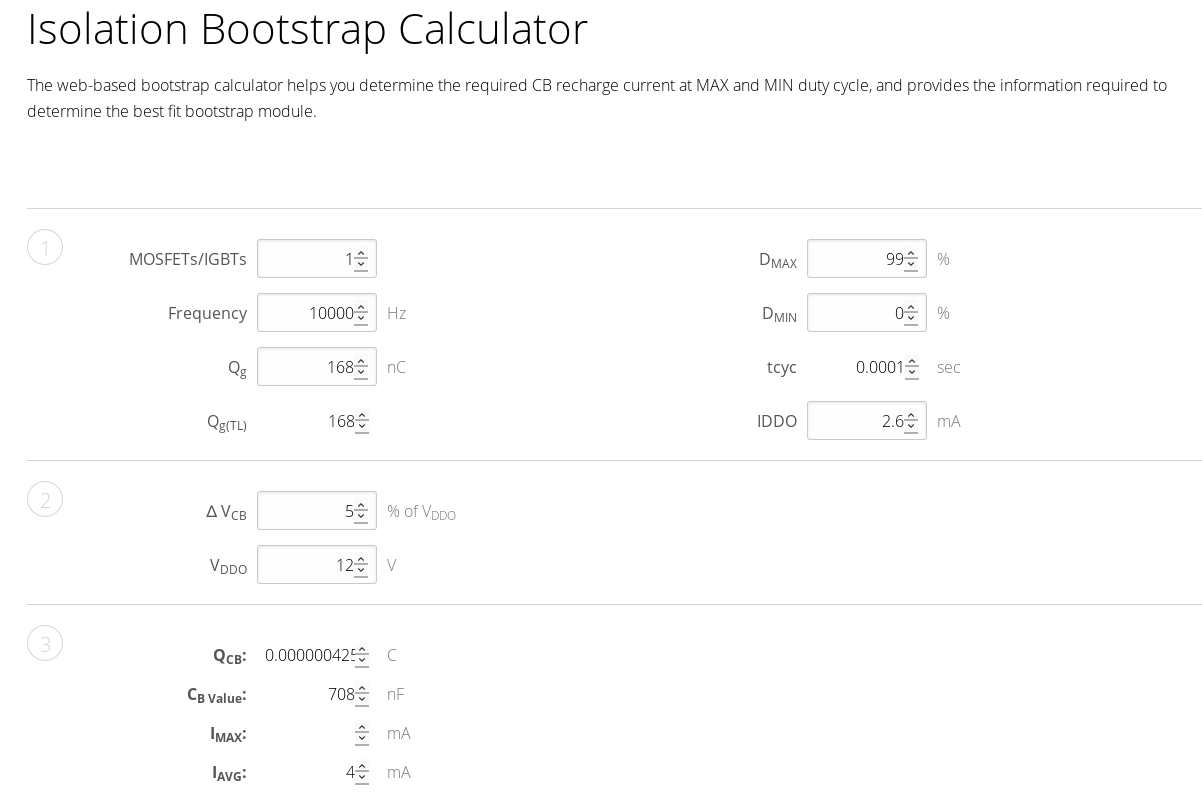
\includegraphics[scale=0.3]{silabs_bootstrap_cap}
			\end{center}
			\caption{Bootstrap capacitor calculator provided by \textit{Silicon Labs} \cite{silabs}.}
			\label{fig:silabsCalc}
		\end{figure}
	
		\subsection{DC-DC Converter}
		To convert 48v into a usable 12v and 5v for the Microcontroller, Gate Driver, etc... I needed a high voltage regulator.  The two types of regulators are linear and switching, and based on the large voltage conversion a switching regulator is the better choice.  \textit{Texas Instruments} TL2575HV switching regulator had the specifications for the job \cite{buck converter}.  In addition it has an adjustable regulator so that I could use the same Integrated Circuit (IC) for both of the conversions.
	
		\subsubsection{5 Volts}
		The 48v to 5v conversion is the harder of the two due do the extensive voltage difference, but running though the calculations given by \cite{buck converter} it is possible.
		
		\vspace{3mm}
		\noindent Known:
		\begin{center}
			\begin{tabular}{ c c c }
			$V_{in} = 48v$ & $V_{out} = 5v$ & $R_{1} = 2k\Omega$ \\
			$I_{load} = 1A$ & $V_{ref} = 1.23v$ & $F_{sw} = 52kHz$
			\end{tabular}
		\end{center}
	
		\noindent Following the sizing steps given by the TL2575HV data sheet \cite{buck converter}:
		\begin{center}
			$R_{2} = R_{1}(\frac{V_{out}}{V_{ref}} - 1) = 6.13k\Omega$ \\
			\vspace{2mm}
			$\epsilon * \tau = (V_{in} - V_{out})*t_{on} = (V_{in} - V_{out}) * \frac{V_{out}}{V_{in}} * \frac{1000}{f_{sw}} = 86.14 V*\mu s$ \\
			\vspace{4mm}
			$86.14 V*\mu s \rightarrow L1 = 330\mu H$ \\
			\vspace{3mm}
			$I_{L_{1}(pk)} = I_{load} + (V_{in} - V_{out}) * \frac{\frac{V_{out}}{V_{in}} * \frac{1}{f_{sw}}}{2*L_{1}} = 1.13 A$ \\
			\vspace{4mm}
			$C_{out} \ge 7758 * \frac{V_{in}}{V_{out} * L_{1}} \rightarrow C_{out} \ge 235.1\mu F \rightarrow C_{out} \approx 1mF$
		\end{center}
		
		
		\subsubsection{12 Volts}
		Write your subsection text here.
	
		\subsection{Microcontroller}
		The STM32F407VG microcontroller was chosen for this project because it contains several features that make PMAC control easier.  The first feature this microcontroller has is automatic dead time insertion \cite{stm32f4 ref manual}.  The second feature is  complementary (low side) wave generation \cite{stm32f4 ref manual}.  In additional to these feature the high clock frequency (168MHz) and built in digital signal processor (DSP) \cite{stm32f4 ref manual} also make this microcontroller a prime choice for this project.
	
		\begin{equation}
		\label{simple_equation}
		\alpha = \sqrt{ \beta }
		\end{equation}
	
	\section{Commutation Techniques}
	Write your section text here.
	
		\subsection{Pulse Width Modulation (PWM) Strategy}
		Up/down counting mode instead of up counting mode to reduce transients so the MOSFETs don't all turn on and off at the same time. Figure \ref{fig:UpCountingMode} shows the up counting mode.  Figure \ref{fig:UpDownCountingMode} shows the 
	
		\begin{figure}[!h]
			\begin{center}
				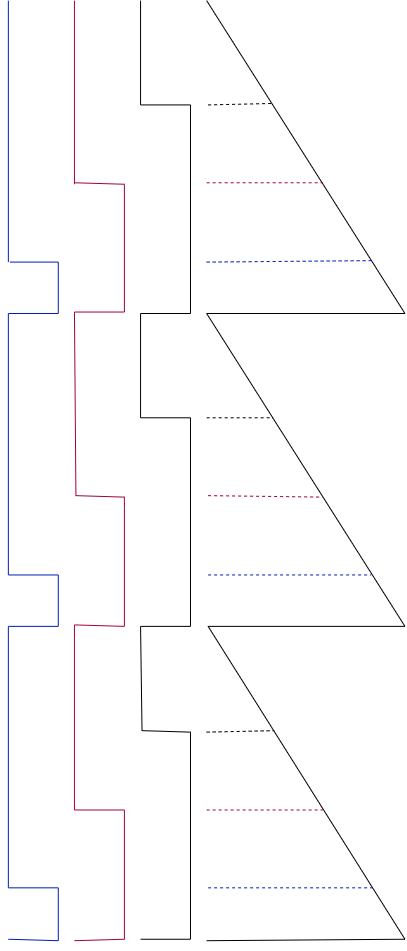
\includegraphics[scale=0.4, angle=90]{UpCountingMode}
			\end{center}
			\caption{Up counting mode for phases A, B, and C.  Turning off all the phases at the same point will induce a transient in voltage and reduce the device's overall electromagnetic compatibility.}
			\label{fig:UpCountingMode}
		\end{figure}
	
	
		\begin{figure}[!h]
			\begin{center}
				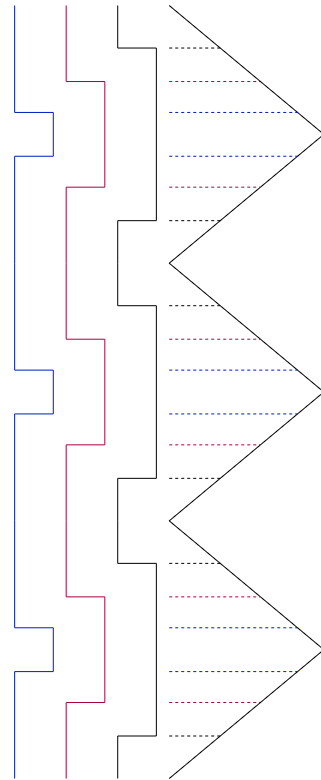
\includegraphics[scale=0.5, angle=90]{UpDownCountingMode}
			\end{center}
			\caption{Up/down counting mode for phases A, B, and C.  This method of PWM reduces electromagnetic interference and also reduces voltage transients by staggering when the MOSFETs turn on and off.}
			\label{fig:UpDownCountingMode}
		\end{figure}
	
		\subsection{Trapezoidal Control}
		Write your subsection text here.
		
		\subsection{Field Oriented Control}
		Write your subsection text here.
	
	\section{Conclusion}
	Write your conclusion here.
	
	\section{Lessons Learned}
	Write your lessons learned here.
	
	
	
	
	\begin{thebibliography}{9}
		\bibitem{Bootstrap Equations}
		Texas Instruments.
		\textit{Bootstrap Circuitry Selection for Half-Bridge Configurations}.
		\\\texttt{http://www.ti.com/lit/an/slua887/slua887.pdf}
		
		\bibitem{silabs} 
		Silicon Labs. 
		\textit{Isolation Bootstrap Calculator}. 
		\\\texttt{https://www.silabs.com/support/isolation-bootstrap-calculator}
		
		\bibitem{buck converter}
		Texas Instruments.
		\textit{TL2575, TL2575HV 1-A Simple Step-Down Switching Voltage Regulators}
		\texttt{http://www.ti.com/lit/ds/symlink/tl2575-12.pdf}
		
		
		\bibitem{stm32f4 ref manual}
		RM0090 Reference Manual
		\textit{STM32F405/415, STM32F407/417, STM32F427/437 and STM32F429/439 advanced Arm-based 32-bit MCUs}
		
		\texttt{https://www.st.com/resource/en/reference\_manual/dm00031020-stm32f405-415-stm32f407-417-stm32f427
			-437-and-stm32f429-439-advanced-arm-based-32-bit-mcus-stmicroelectronics.pdf}
		
		
	\end{thebibliography}
	
	
	
\end{document}